% =====================================================================
% CHAPTER 4 -- Summary of: A. F. Vaquero et al., IEEE OJAP, 2026 [Vaquero2026]
% =====================================================================
\section*{CHAPTER 4. NEAR-FIELD SES FOR INDOOR COVERAGE}
\addcontentsline{toc}{section}{\numberline{}CHAPTER 4. NEAR-FIELD SES FOR INDOOR COVERAGE}
\setcounter{section}{4}
\setcounter{subsection}{0}
\setcounter{equation}{0}
\setcounter{theorem}{0}
\setcounter{figure}{0}
\setcounter{table}{0}

\subsection{Problem}
RISs can follow users, but large-scale deployment is limited by their power supply and by the channel-state information and signalling they need~\cite{Vaquero2026}. Passive SESs need neither, which suits them to \emph{static} blind spots, a common problem indoors at mmWave. To capture enough power, however, an SES must span tens of wavelengths, and its far-field (Fraunhofer) region only starts at
\begin{equation}\label{eq:ch4-fraunhofer}
d_F = \frac{2D^2}{\lambda},
\end{equation}
where $D$ is the largest dimension of the aperture and $\lambda$ the wavelength. For a $30\lambda \times 30\lambda$ SES at about 30~GHz ($D \approx 0.42$~m along the diagonal, $\lambda = 10$~mm), \eqref{eq:ch4-fraunhofer} gives about 36~m, in line with the roughly 40~m quoted in~\cite{Vaquero2026}. Indoor users therefore sit in the near field, where the usual plane-wave, far-field design does not hold. Cost is a second constraint: cheap single-layer patch cells cannot provide a full $360^\circ$ phase cycle.

\subsection{Contributions and Methodology}
Vaquero \textit{et al.}~\cite{Vaquero2026} design, build and test an SES that removes a static blind spot in a realistic indoor scenario at 24.45~GHz. They make three contributions:
\begin{enumerate}
    \item a near-field synthesis that uses the actual field radiated by the BS and the limited phase range of the unit cell;
    \item RF validation in a real laboratory;
    \item an end-to-end near-field communication (NFC) link evaluated with the error vector magnitude (EVM) and the symbol error rate (SER).
\end{enumerate}
\begin{itemize}
    \item \textbf{Unit cell.} The cell is a square patch on a single DiClad~880 layer ($\varepsilon_r = 2.3$, $\tan\delta = 0.005$, $h = 0.786$~mm) with a 4.93~mm ($0.4\lambda_0$) period. A spectral-domain method of moments gives losses better than $-0.4$~dB ($-0.15$~dB on average) and about $300^\circ$ of phase, of which about $270^\circ$ is nearly linear.
    \item \textbf{Base station.} The BS is emulated by a $400 \times 400$~mm ($32.34\lambda_0$) reflectarray with $81 \times 81$ elements and a 15~dBi horn feed. Its measured gain is 32.4~dBi at 24.45~GHz (34.81~dBi simulated), and it illuminates the SES from about 3.6~m.
    \item \textbf{SES synthesis.} The SES has the same $400 \times 400$~mm size as a reference metal plate.
    \begin{itemize}
        \item Its phase comes from a generalized Intersection Approach that imposes the field specifications directly in the near field.
        \item A Levenberg--Marquardt optimizer adjusts the phases, with an extra projector that clips every phase to the $270^\circ$ range the cell can provide.
        \item The SES redirects the beam to $46^\circ$ in azimuth and widens it to cover $\pm 5^\circ$ (azimuth) $\times$ $\pm 3^\circ$ (elevation) around the blind spot.
        \item A two-stage synthesis tightens the ripple target from 2~dB over 75\% of the region to 1.5~dB over 100\%.
    \end{itemize}
    \item \textbf{NFC testbed.} Two USRP N210 software-defined radios with mmWave mixers and amplifiers transmit single-carrier subchannels of 6.5~MHz spaced by 8~MHz (50 subchannels in 400~MHz). The receiver is a monopole antenna 1.5~m above the floor.
\end{itemize}
The spectral efficiency of this architecture is~\cite{Vaquero2026}
\begin{equation}\label{eq:ch4-se}
\eta = \frac{5}{8}\log_2 M \quad \text{(bit/s/Hz)},
\end{equation}
where $M$ is the constellation order. The factor $5/8$ comes from the 5~Msymbol/s carried by each 8~MHz subchannel (10~Msample/s, two samples per symbol, roll-off 0.3 and a 1.5~MHz guard band).

\subsection{Limitations of the Approach}
\begin{itemize}
    \item The cheap single-layer cell offers only $270^\circ$ of usable phase. The synthesis respects this limit, but the limit still constrains the achievable patterns.
    \item The laboratory fixes the scenario: one blind spot, one BS position, and results reported for x-polarization only. The BS is a passive reflectarray emulating a massive-MIMO station.
    \item The link test uses narrow 6.5~MHz subchannels (limited by the USRP sampling rate), no channel coding, and commercial hardware with visible phase noise.
\end{itemize}

\subsection{Results and Evaluation}
Fig.~\ref{fig:ch4-nearfield} compares the measured near field of the SES and of the metal plate over a $1 \times 1.6$~m$^2$ plane (1749 points, 15~mm step) at 24.25, 24.45 and 24.65~GHz~\cite{Vaquero2026}.
\begin{itemize}
    \item With the SES, the peak-to-peak ripple at the 4.6~m synthesis plane is below 1.5~dB, and the spot keeps the same shape over at least 1~m in depth. At the border of the region ($y = 2$~m) the ripple increases but stays within 5~dB.
    \item The metal plate reflects only specularly. Its spot is just 2--3$^\circ$ wide, with 5--10~dB of ripple, and it shifts with frequency because of the BS beam squint.
\end{itemize}
The difference comes from the synthesis. A flat reflector keeps the very narrow BS beam (simulated 3-dB beamwidth below $\pm 1^\circ$), whereas the SES widens and re-points it and holds the pointing stable across the band.

\begin{figure}[!htbp]
    \centering
    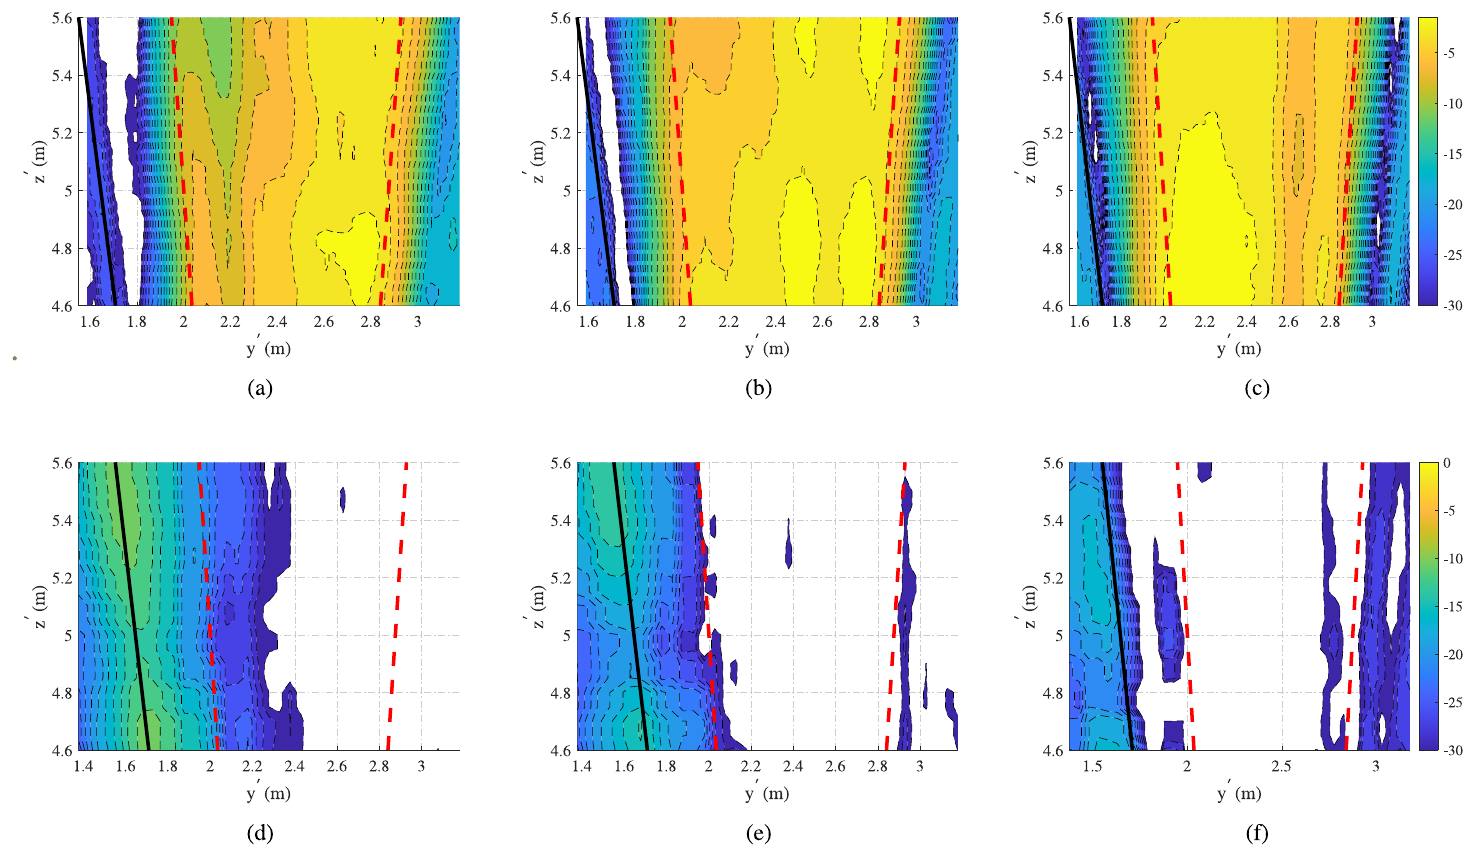
\includegraphics[width=\textwidth]{Images/ch4_vaquero_fig13.png}
    \caption[Measured near-field coverage of the SES and of a metal plate]{Measured near-field pattern (dB) of (a)--(c) the SES and (d)--(f) a metal plate of the same size at 24.25, 24.45 and 24.65~GHz (x-polarization, normalized to the maximum coverage at 24.45~GHz); red lines bound the target angular coverage and the black line marks the specular direction (adapted from~\cite{Vaquero2026}).}
    \label{fig:ch4-nearfield}
\end{figure}

Table~\ref{tab:ch4-link} reports the link measurements at 24.45~GHz, with about 0~dBm fed to the transmit antenna.
\begin{itemize}
    \item Through the SES, 64-QAM reaches an EVM of $-29.9$~dB, with SER below $10^{-5}$, at the centre of the spot. At its 3~dB edge the EVM is $-27.5$~dB.
    \item Through the metal plate, the same position only supports QPSK, with an EVM of $-13.2$~dB.
    \item The uplink is 0.5--1.5~dB worse in EVM than the downlink, because the active hardware (e.g., the power amplifier) is not reciprocal.
    \item At the spot centre the EVM saturates: 3~dB more received power improves it by only 2.4~dB, because phase noise and nonlinear distortion dominate.
    \item With 64-QAM, \eqref{eq:ch4-se} gives $\eta = 3.75$~bit/s/Hz, i.e., 1.5~Gbit/s over the 400~MHz channel at an uncoded SER below $10^{-4}$.
\end{itemize}

\begin{table}[!htbp]
    \centering
    \caption[Measured near-field link performance]{Measured link performance at 24.45~GHz; $P_{\mathrm{design}}$ is the centre of the synthesis plane and $P_{\mathrm{aperture}}$ the point where the field has dropped by 3~dB~\cite{Vaquero2026}.}
    \label{tab:ch4-link}
    \small
    \begin{tabular}{l l l l c c}
        \toprule
        Reflector & Modulation & Link & Position & EVM (dB) & SER \\
        \midrule
        SES & 64-QAM & downlink & $P_{\mathrm{design}}$ & $-29.9$ & $< 10^{-5}$ \\
        SES & 16-QAM & uplink & $P_{\mathrm{design}}$ & $-28.4$ & $< 10^{-5}$ \\
        SES & 64-QAM & downlink & $P_{\mathrm{aperture}}$ & $-27.5$ & $< 10^{-4}$ \\
        Metal plate & QPSK & downlink & $P_{\mathrm{aperture}}$ & $-13.2$ & $< 10^{-4}$ \\
        \bottomrule
    \end{tabular}
\end{table}

\subsection{Open Issues and Future Directions}
The authors note that the method also covers wider incidence ranges, larger reflection angles, circular polarization or polarization conversion, and scenarios with several SESs or metallic scatterers; only the unit cell has to change~\cite{Vaquero2026}. Several points remain to be demonstrated:
\begin{itemize}
    \item full-band links using many subchannels at once;
    \item coded transmission and the effective data rate it delivers;
    \item blind spots that change over time (moving users or obstacles), which a passive SES cannot follow.
\end{itemize}
